\anhang{Experteninterview Ralph B.}\label{anhang:interview-ralph-24.03.2021}
\begin{table}[H]
\begin{tabularx}{\textwidth}{|l|X|}
\hline
    Datum                  & 24.03.2021 \\ \hline
    Thema                  & Initiales Anforderungsinterview \\ \hline
    \begin{tabular}[c]{@{}l@{}}Teilnehmende,\\ Position\end{tabular} & \begin{tabular}[c]{@{}l@{}}Lukas Fruntke, Verfasser\\ Ralph B., Bereichsverantwortlicher - \ac{rnd}\end{tabular}\\ \hline
\end{tabularx}
\end{table}
\newcommand{\RB}{\textbf{Ralph B.:}~}

\LF Herzlichen Dank Ralph, für deine Bereitschaft zum Interview. Beginnend möchte ich dich fragen, was deine Rolle/Tätigkeiten innerhalb der SPIRIT/21 sind und wie du mit Architekturen zu tun hast.

\RB Meine Rolle in der SPIRIT hat sich schon ein paar mal gewandelt. Aktuell bin ich für den Bereich Lead \ac{rnd} Verantwortlicher für Forschung und Entwicklung. Als Vorsitzender des Tech- und Architekturboards bin ich für die technologische Qualifizierung von Entwicklungsthemen verantwortlich. Genauso koordiniere ich auch den Einsatz von bestimmten neuen Technologien in den einzelnen Solutions.

\LF Verstehe. Wo siehst du denn Anwendungsgebiete von Referenzarchitekturen in Richtung Zeitreihendatenverarbeitung? 

\RB Welche Architekturen siehst du denn da im Scope? Softwarearchitekturen, oder Infrastrukturachitekturen oder eine andere Architektur?

\LF Ich denke an technische Architekturen, die einen Teil Software und Infrastrukturkomposition umfassen, best practices und eine Art Referenzvorgehen sind \enquote{wie löse ich dieses wiederkehrende Problem, dass immer wieder auftaucht}? Speziell in Richtung Cloud und \ac{AWS} gesehen.

\RB Gut, \ac{AWS} Cloud sehe ich jetzt firmenweit betrachtet nur als ein Teilthema von vielen. Generell zählen für mich da organisatorische und fachliche Richtlinien/Konzepte mit herein. Das geht über die wiederverwendbare technische Lösung hinaus. Vielleicht sollten auch Problem adressiert werden, die momentan nicht akut sind, aber in Zukunft wichtig werden könnten. Generell kann man nicht von einer schlechten Architektur oder einer schlechten Referenzarchitektur sprechen. Klassifizierung in gut oder schlecht ist schwierig. Stattdessen muss man schauen, ob die Architektur auf den Usecase passt oder nicht. 

\LF Konkret Richtung Zeitreihendaten gedacht - wo siehst du konkret die Anwendungsgebiete, wo eine Referenzarchitektur unterstützen könnte?

\RB Das ist generisch immer ein wenig schwierig. Es kommt auf den Anwendungsfall an. Bei Datenerfassung bei \ac{IoT}-Daten muss das Kriterium angelegt werden, ob sehr viele Daten in kurzer Zeit erfasst werden können. Ist die Lösung skalierbar? Wichtig ist aber auch das Ausgeben der Daten: müssen diese instant bereit stehen, oder habe ich da einen Zeitpuffer von fünf Sekunden, bis diese wieder bereit stehen müssen? Wenn ich Daten gespeichert habe, wie lange braucht es die zu lesen? Wo sind Bottlenecks etc.? Im \ac{IoT} Bereich ist speziell der Durchsatz, also die Messages pro Sekunde, die kommen könnten ein Problem, weil jeder Sensor einen Wert sendet, der dann gespeichert werden will. Das hat dann auch mit Verfügbarkeit zu tun - wie bekomme ich die Datenbank dahinter 100\% verfügbar? Die konkreten Anforderungen sind dabei immer unterschiedlich. Wenn man jetzt z.B. \ac{LoRaWAN} Sensordaten hat von 20.000 Sensoren, die alle x Sekunden Daten senden. Kann meine Datenbank diese speichern? Und wenn ich dann einen Report möchte einmal pro Woche, dann möchte ich nicht lange warten, sondern schnell in den Daten navigieren können.

\LF Wir haben ja jetzt schon ein wenig Richtung \ac{IIoT} Daten geschaut. Speziell die Problematik mit den Auswertungen ist da wichtig. Entsprechend dem Datenhalbwertszeitmodell hat es ja drei verschiedene Entscheidertypen, die Daten in unterschiedlicher Zeit benötigen und Entscheidungen treffen. Taktische Entscheider brauchen Daten sehr schnell und trifft auch schnell Entscheidungen. Operative Entscheider brauchen Daten nicht unbedingt nahe Echtzeit und haben einen erweiterten Entscheidungshorizont, auf Tage oder Wochen. Strategische Entscheider haben einen wesentlich größeren Entscheidungshorizont gleichzeitig aber auch geringere Anforderungen an die \enquote{Echtzeitigkeit} der Daten. Welche siehst du denn als am wichtigsten an oder für welche würdest du im \ac{IoT} Bereich optimieren?

\RB Ich denke die sind alle gleich wichtig. Im operativen Entscheidungsmodus sollten die Entscheidungsregeln idealerweise automatisiert sein. Einen ausgelösten Feuermelder mit einer Email an einen Verantwortlichen zu koppeln, macht weniger Sinn, als beispielsweise die Werksfeuerwehr zu rufen. Bei unseren bisherigen Projekten ist Latenz nicht so wichtig - da die Geräte bei Bedarf Nachrichten senden oder in Intervallen von 50/60 Sekunden. Latenz wird aber wieder wichtig, wenn man beispielsweise einen Wassersensor hat, der eine Aktion in der Businesslogik auslöst, die das Wasser bei Kontakt abstellt. Von den historischen Daten kann man ein Dashboard befüllen, wo ein Entscheider einmal die Woche drüberschaut und Entscheidungen trifft. Dann gibt es noch langfristige Usecases - Billing Daten beispielsweise interessieren den Kunden nur einmal im Monat.

\LF Okay, verstehe. Ein bisschen von der Technik weg - es gibt ja Qualitätskriterien zu Referenzarchitekturen - die hatte ich dir schon gesendet. Wie siehst du denn die?

\RB Ich bin da noch eher klassisch. Wenn du jetzt die ISO 9126 anschaust für Qualität von Softwaresystemen (\textit{siehe \autoref{abb:ISO9126}}), hast du noch ein paar andere Kriterien. Was ist denn zufriedenstellende Qualität? Wenn der Kunde zufrieden ist, ist es dann zufriedenstellend? Qualitätsmerkmale sind immer schwammig, weil es nicht \enquote{die Qualität} gibt. Es gibt nur eine passende Architektur, die eine passt besser, die andere schlechter. Qualität ist nicht absolut, sondern relativ anhand von Kriterien. 

\begin{figure}[H]
\centering
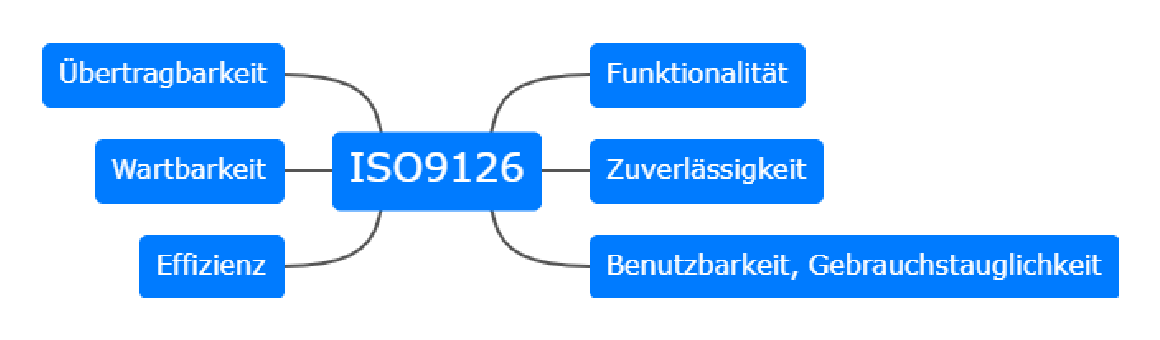
\includegraphics[width=\textwidth]{graphics/ISO-9126.pdf}
\caption[Qualitätskriterien nach ISO 9126]{Qualitätskriterien nach ISO 9126.\footnotemark}
\label{abb:ISO9126}
\end{figure}
\footnotetext{Mit Änderungen entnommen aus: \cite{Johner.2018}}

\LF Ja, für mich geht es darum zu erfahren, welche Kriterien da für den maximierten Nutzen für unsere Zielstakeholder am wichtigsten sind.

\RB Übertragbarkeit zwischen Usecases ist wichtig. Gleichzeitig muss man aber schauen, dass man sich nicht zu sehr fokussiert auf ein Qualitätskriterium. Wenn man beispielsweise bewusst auf single-instance Datenbanken verzichtet und diese immer im Cluster errichtet, erhöht das die Zuverlässigkeit, sprengt aber vielleicht den Preisrahmen des Usecases. 

\LF Da möchte ich mit den Variationspunkten ansetzen, wo ich Entscheidungsoptionen aufzeige wie man die Referenzarchitektur instanziieren kann.

\RB Das Problem ist ja, dass man meistens mit mehr Qualitätskriterien, die man berücksichtigt das Resultat teurer wird.

\LF Da macht das KISS Prinzip dann eher Sinn, oder?

\RB Genau. Der Kunde sollte halt immer den Mehrwert sehen hinter den extra Features die man implementiert. Achte auch auf die Zuverlässigkeit und Modifizierbarkeit. 

\LF Werde ich. In meiner Bachelorarbeit konstruiere ich Referenzarchitekturen für Batch-Verarbeitung \`{a} la \ac{OLAP} und für Echtzeitverarbeitung.

\RB Okay, versteh ich. Da musst du aber den Reifegrad beachten der Architektur - ob die sich schon bewährt hat. Die meisten Referenzarchitekturen entstehen ja aus Mustern, die sich in mehreren Projekten bewährt haben.

\LF Genau, ich kenne aus der Literatur zwei Zugänge zur Referenzarchitektur. Das ableiten von Mustern aus bewährten Projekten oder das man induktiv eine best-practice Architektur von neuen Produkten/Diensten ableitet. Momentan sind die Clouddienste uns ja noch eher unbekannt in diese Richtung, deshalb würde ich gerne mit dem zweiten Ansatz Referenzarchitekturen erarbeiten.

\RB Das schwierige ist, das spezifisch zu machen. Da ist ja ein Spannungsfeld zwischen Allgemeingültigkeit und Überanpassung auf einzelne Usecases.

\LF Ja, da haben wir uns meinem Dimensionenmodell ja schon etwas angenähert, da geht es ja auch um die Allgemeingültigkeit. Da wäre meine Frage, wie du die einzelnen \enquote{Richtungen} einschätzen würdest.

\RB Auch deine Referenzarchitektur muss sich weiterentwickeln und in eine Lösung überführt werden können. Nur als Lösung ist die Referenzarchitektur dann auch marktgängig. Ganz früher waren Softwarearchitekturen nur Designpatterns. Da hat man den Entwicklern gesagt \enquote{hey macht mal, setzt mal um}. Dafür haben wir heute keine Zeit. Wir brauchen die Wiederverwendung. 

\LF Verstehe. Von der Allgemeingültigkeit, so wie ich das jetzt verstanden habe wäre das so ziemlich in der Mitte. Es darf nicht zu spezifisch sein, es darf aber auch nicht zu generisch sein, weil es dann nicht marktgängig ist, oder?

\RB Eine Architektur ist ja klar nicht marktgängig sondern die implementierende Lösung. Aber die Architektur muss die Lösung marktgängig machen. Dazu muss sie die Kundenkriterien berücksichtigen. Sei es Benutzbarkeit, Effizienz, Übetragbarkeit, Funktionalität, ... (\textit{siehe \autoref{abb:ISO9126}}). Je nach Kunde benötigt man eine extrem hohe Performance, oder die Fähigkeit viele Daten aufzubewahren. Da kann dann beispielsweise ein Cluster oder ein \ac{AWS} Service die Lösung sein.

\LF In Richtung \ac{AWS} wollte ich ja generell schauen in der Bachelorarbeit. Weil die Services eben managed sind, sind sie ja auch autoskalierend meistens.

\RB Da musst du aber auch aufpassen. Elasticsearch ist beispielsweise ja in Teilen autoskalierend. Oder der AWS IoT Core Hub der garantiert eine Billion Messages, das muss man erstmal selber hinbekommen. Diese Probleme sind weg, aber sie haben auch Services, wo du selber skalieren musst. 

\LF Ja, Kinesis Data Streams ist beispielsweise einer der Dienste wo man selber Shards nachprovisionieren muss, damit man skalieren kann.

\RB Da muss man halt aufpassen. Wo sind die Limitierungen, was geht.

\LF Das werde ich in der Arbeit mit ausloten.

\RB Hier (\textit{\autoref{abb:ISO9126}}) siehst du die ISO 9126. Die Norm ist relativ alt, aber passt eigentlich immer noch. Interessant ist dabei der Punkt Übertragbarkeit. Das finde ich, ist bei \ac{AWS}-Services etwas, das thematisiert werden sollte. Es ist unbestreitbar, dass die Benutzbarkeit von \ac{AWS}-Services gut ist, dass die Effizienz und Zuverlässigkeit ziemlich gut sind. Die Funktionalität ist meistens auch nicht schlecht, aber mit der Übertragbarkeit haben wir meistens ein Problem.

\LF Das ist ja aber immer bei so managed services ein Problem.

\RB Aber man muss da drastisch unterscheiden und das ist für mich ein Kernunterscheidungsmerkmal. Die Übertragbarkeit ist trotzdem bei vielen Kunden wichtig. Es spricht jetzt nichts gegen \ac{AWS}, wenn du beispielsweise den Elasticsearch service nimmst hast du ja ein Standard Elasticsearch. Das kannst du einfach übertragen.

\LF Es gibt ja bei \ac{AWS} verschiedene Services. Sowohl native, als auch managed Kafka oder ähnliches.

\RB Genau managed Kafka, oder es gibt jetzt auch neuerdings managed OpenShift - coole Sache. Die Frag ist  halt, inwiefern ist es standardkonform und inwiefern nicht mehr. Das ist ein wichtiger Aspekt finde ich. Wenn man jetzt nur die Cloud betrachtet eher irrelevant, also wenn jemand sowieso nur \ac{AWS} machen will, dann ist es egal.

\LF Ja, das wäre eher die Zielsetzung meiner Arbeit gewesen.

\RB Ja, schwierig ist da nur, dass sich allein der verantwortliche IT-Leiter beim Kunden ändern muss, der \ac{AWS} blöd findet und alles auf Azure packen möchte. Dann wäre es doch wichtig zu wissen, ob die Kafka nimmst, was man woanders auch bekommt, oder ob du eine properitäre Lösung verwendest. Das ist schon ein Kriterieum, was man betrachten sollte.

\LF Übertragbarkeit werde ich auf jeden Fall mit anschauen. Ich hab schon einige Alternativen ausgemacht, wo man entweder properitäre, \ac{AWS}-native Dienste verwenden kann, oder managed open source Dienste wie Kafka. Noch kurz zu dem Dimensionsmodell. Zusammenfassend wäre die subjektive Allgemeingültigkeit ziemlich in der Mitte, die Anwendbarkeit möglichst hoch. Wie siehst du die Dekompositionstiefe?

\RB Das ist immer eine gute frage. So tief wie nötig, aber nicht tiefer. Da gab es Versuche, beispielsweise arc42 vollständig auszufüllen. Die Diskussion hatten wir schon, das halte ich für nicht gut. Dokumentation generell soltle da eintreten, wo es Abweichungen gibt, oder wo es kompliziert wird. Ansonsten sollte man auf einer hohen Ebene agieren.

\LF Von den Zahlen her also 2/3 in der Mitte?

\RB Genau das. Das Problem ist, Architekturen sind für viele ja eher Neuland. Man muss sich da teilweise ran tasten. Die Architekturwerkzeuge helfen beim Bauen einer Lösung. Es ist beispielsweise bei einem Hammer und Nagel immer noch abhängig vom Handwerker, ob der Nagel gerade in der Wand steckt. Eine Architektur, die nur ein Bauplan sind, aber nicht vermitteln warum man was macht sind ein Problem.

\LF Da hätte ich versucht die Tradeoffs ensprechend zu erklären, die ich eingehe.

\RB Genau. Ich muss leider weiter.

\LF Okay, dann vielen Dank für das Interview.

\RB Gerne, ich hoffe es hat dir geholfen.
